\testCom
{%Номер задачи
	3.107
}
{%Условие
	условие
}
{%Дано
	дано
}
{%Найти
	найти
}
{%Решение
	%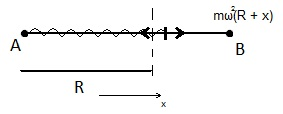
\includegraphics[height=30mm]{3_33.jpg}\\
	Очевидно, что $A_{tr} = -2 \int\limits_{-a}^{a} F_{tr}\, dx = - 2 \int\limits_{-a_m}^{a_m} N_{tr} \, d\varphi$\\
	$I \der{\varphi}{t}{2} + k \der{\varphi}{t}{} + I \omega_0^2 \varphi = N(t)$, тогда \\
	$A_{тр} = 2 k \int\limits_{-\varphi_m}^{\varphi_m} \der{\varphi}{t}{}\, d\varphi = 2  \int\limits_{-\varphi_m}^{\varphi_m} (N(t) - I \ddot \varphi - I \omega^2 \varphi) d \varphi = $\\
	$= 2 \int\limits_{\frac{\pi + \alpha}{\omega}}^{\frac{2 \pi + \alpha}{\omega}} (N(t) - I \varphi (\omega^2 - \omega^2)) \dot \varphi dt =$\\
	$= 2 \omega \int\limits_{\frac{\pi + \alpha}{\omega}}^{\frac{2 \pi + \alpha}{\omega}} N_m \cos \omega t \varphi_m \sin (\omega t - \alpha) dt =$\\
	$= 2 \omega N_m \varphi_m \int\limits_{\frac{\pi + \alpha}{\omega}}^{\frac{2 \pi + \alpha}{\omega}} (\cancelto{0}{\cos \omega t \sin \omega t} \cos \alpha - \cos^2 \omega t \sin \alpha) dt =$\\
	$= -\cancel 2 \cancel \omega N_m \varphi_m \frac{\pi \sin \alpha}{\cancel 2 \cancel \omega} = - \pi N_m \varphi_m \sin \alpha$\\
}

